\documentclass{article}
\usepackage{graphicx} % Required for inserting images
\usepackage{amsmath}
\usepackage{mathalfa}
\usepackage{blindtext}
\usepackage[letterpaper, portrait, margin=0.75in]{geometry}
\usepackage{amssymb}
\usepackage{epsf, subfigure, verbatim, epsfig}
\usepackage{fancyhdr}
\usepackage{calc}
\usepackage{ifthen}
\usepackage{layout}
\usepackage{fancybox}
\usepackage{eurosym}
\usepackage{tabularx}
\usepackage{xspace}
\usepackage{dsfont,mathrsfs}
\usepackage{amssymb}
\usepackage{theorem}
\usepackage{multicol}
\usepackage{float}

\title{Homework 1 \\ \large MATH 476}
\author{Ahad Jiva}
\date{April 8, 2025}

\begin{document}

\maketitle
\section*{Exercise 1} 
\begin{flushleft}
    \textbf{Forward Contract Payoff}
    \begin{enumerate}
        \item The payoff from a long position (buying the asset) in a forward contract is $S_T - K$.
        \item The payoff from a short position (selling the asset) in a forward contract is $K - S_T$.
    \end{enumerate}
\end{flushleft}
\section*{Exercise 2}
\begin{flushleft}
    \textbf{Forward Contract on Stock Index} \\
    We know the current price is \$1000 and the 6-month forward price is \$1020.
    \begin{enumerate}
        \item If the price is \$950 in 6 months, the long position will lose \$70 (950 - 1020).
        \item If the price is \$1200 in 6 months, the long position will gain \$180 (1200 - 1020).        
    \end{enumerate}
    The forward contract allows for a profit if the value of the asset increases after 6 months, without having to actually own the asset.
    \\ Payoff Diagram:
    \begin{center}
        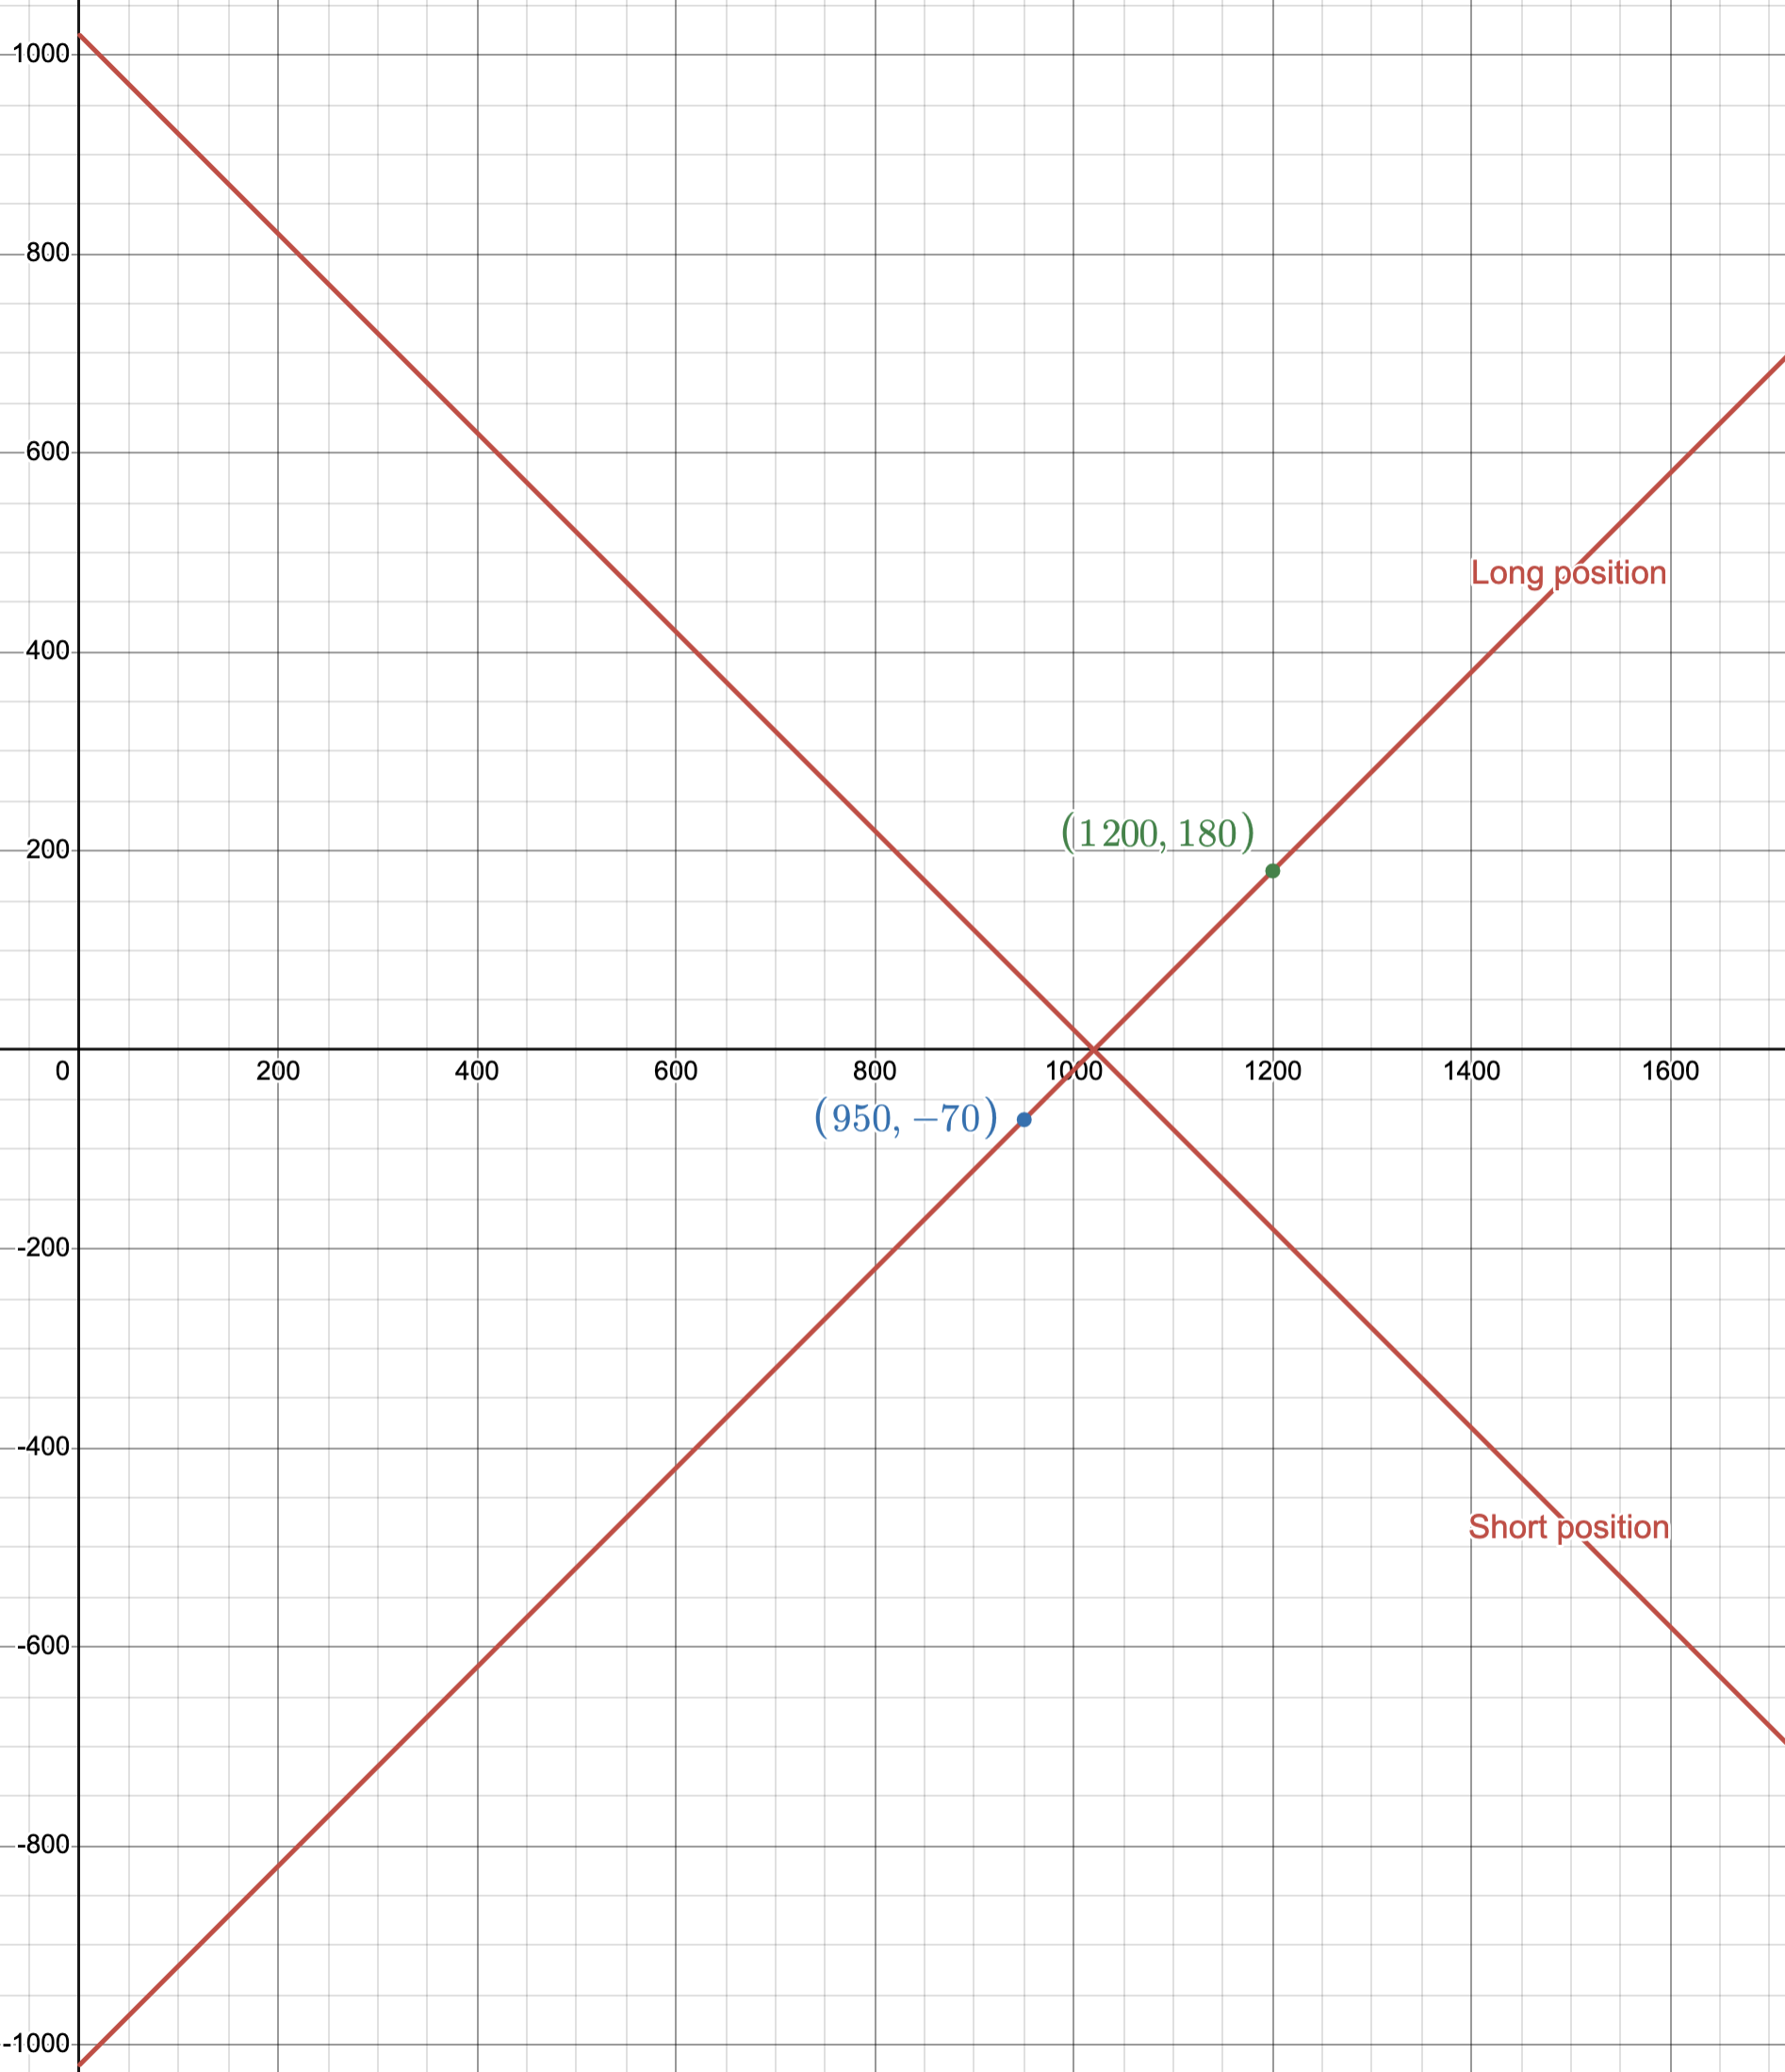
\includegraphics[width=0.5\textwidth]{ex2.png}
    \end{center}
\end{flushleft}

\section*{Exercise 3}
\begin{flushleft}
    \textbf{Payoff Diagrams for Forward Contract}
\end{flushleft}
\begin{center}
    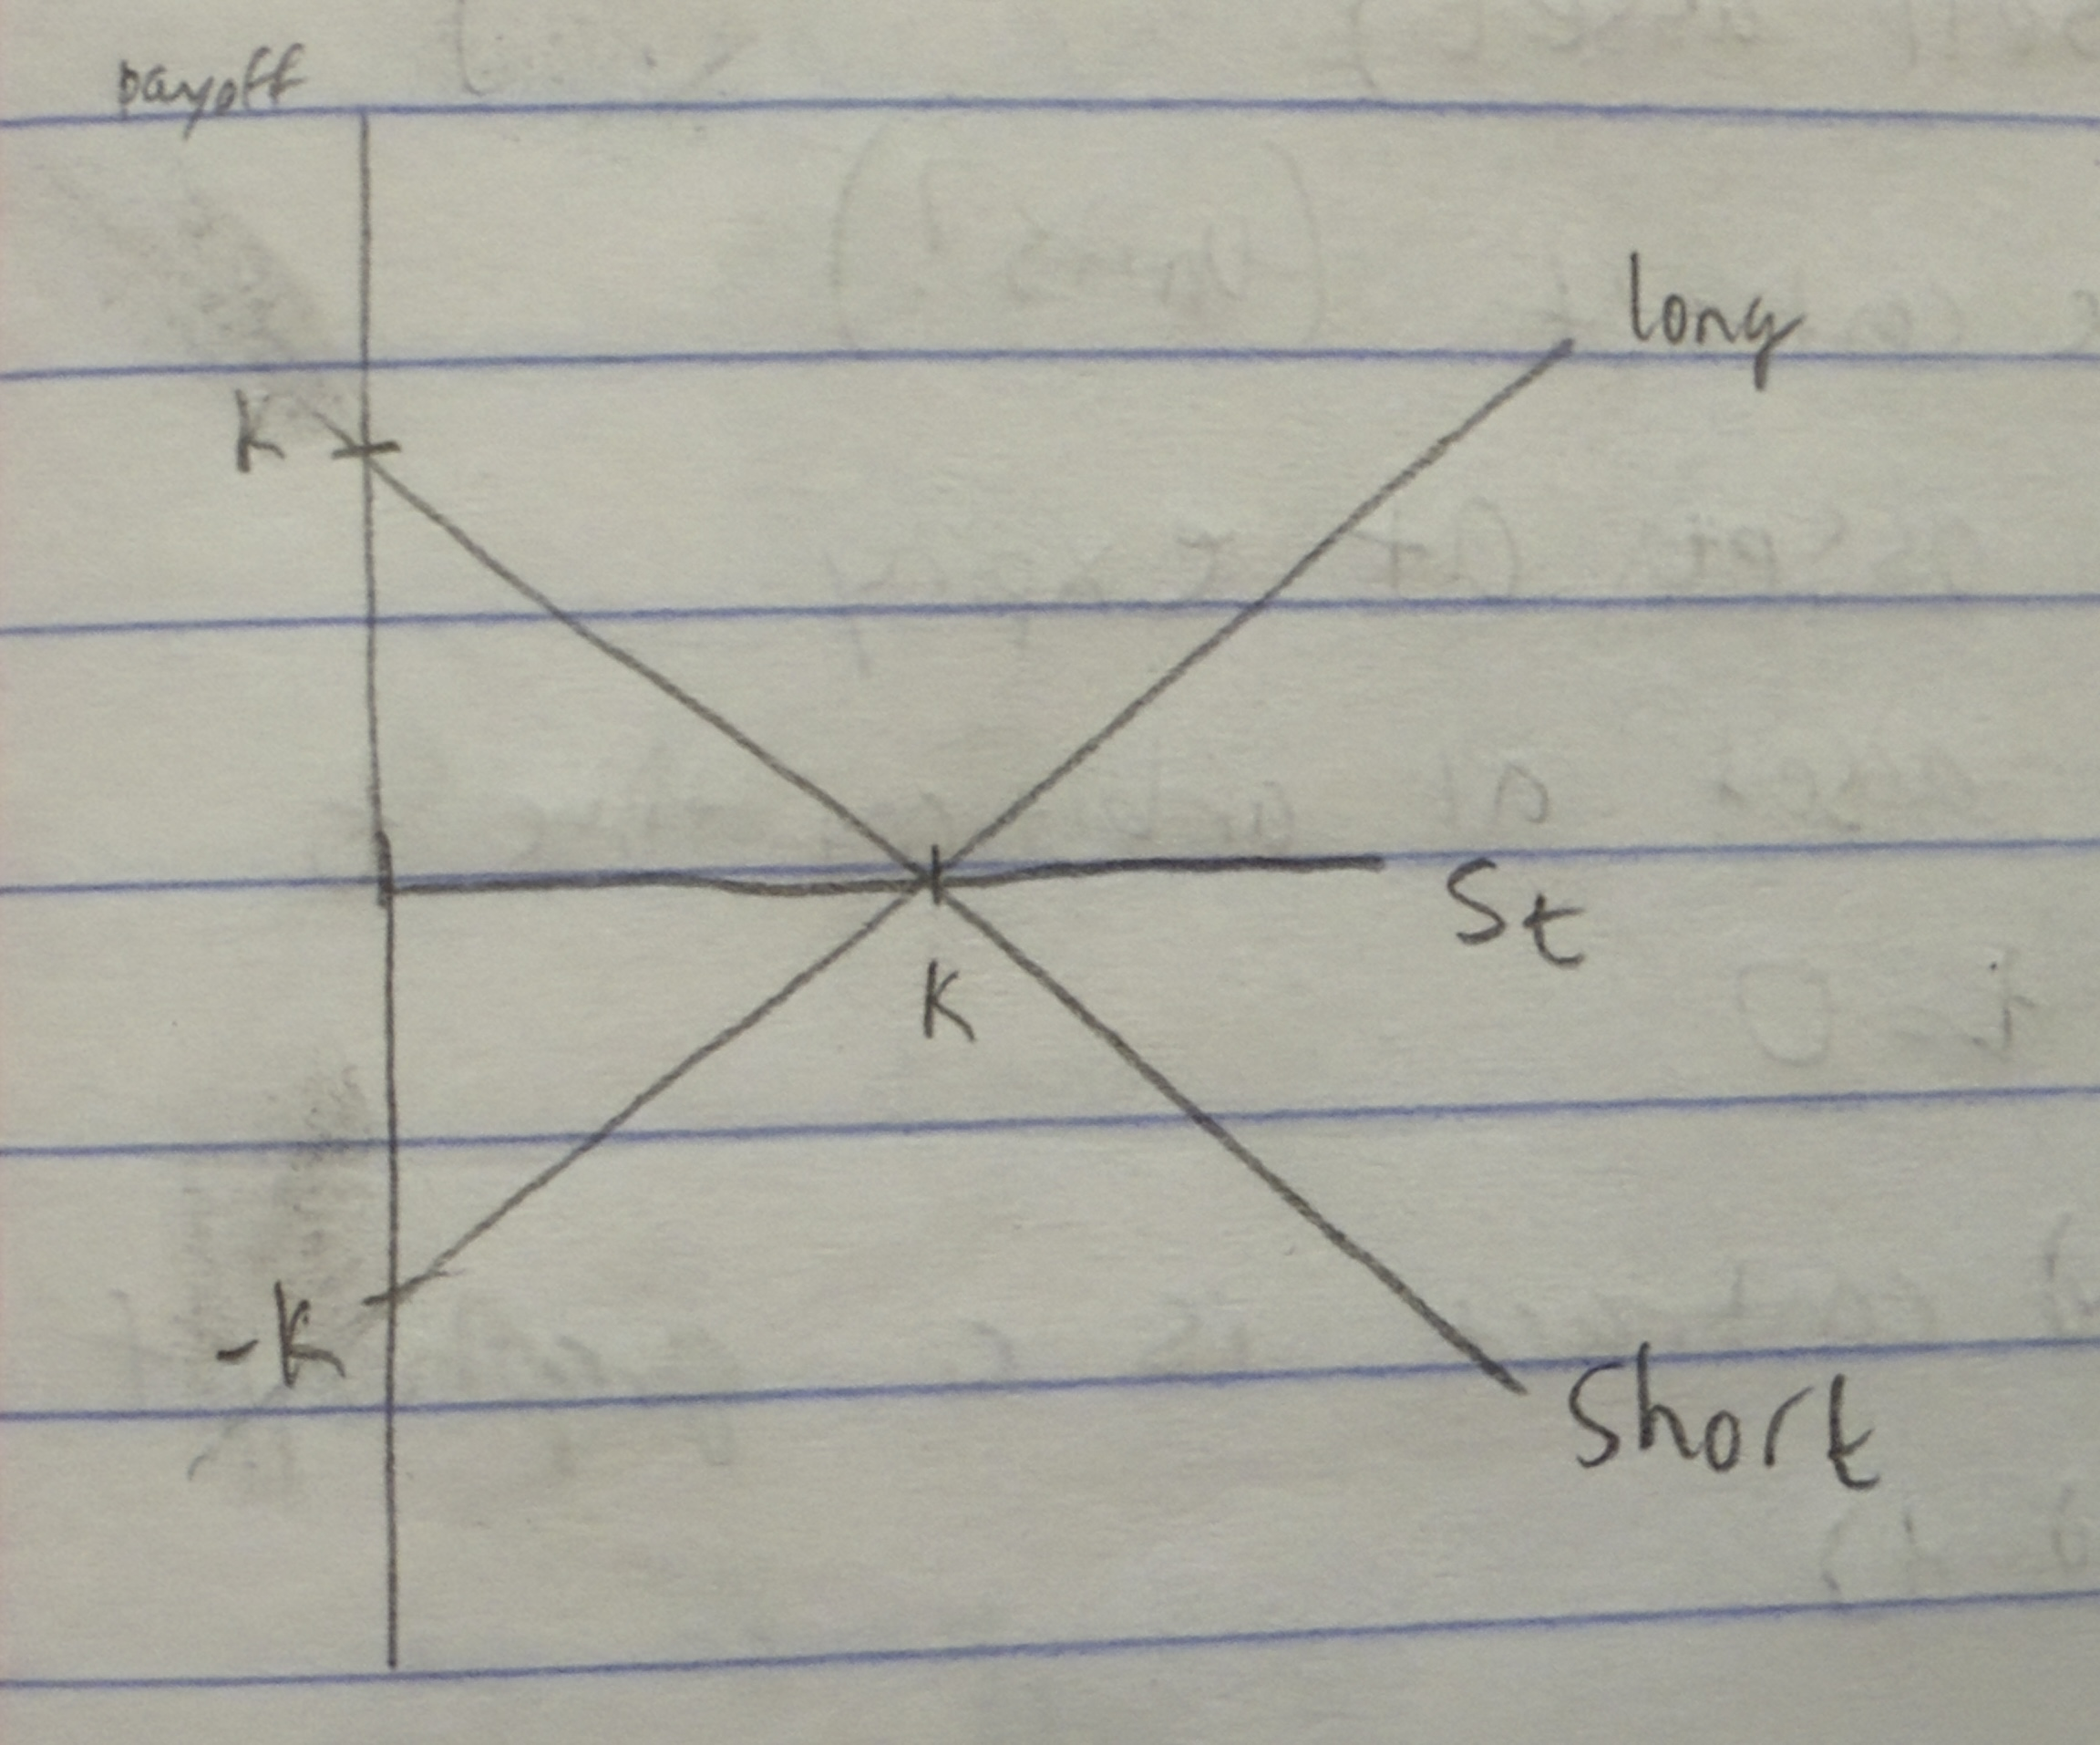
\includegraphics[width=0.5\textwidth]{ex3.jpg}
\end{center}

\section*{Exercise 4}
\begin{flushleft}
    \textbf{Forward Contract on Foreign Exchange} \\
    The bank agrees to a 6-month forward contract to purchase 1 million GBP in 6 months.
    \begin{enumerate}
        \item If the spot price is 1.3000 in 6 months, the bank will make $(1.3000 - 1.2230) \cdot 1000000 = \$77000$.
        \item If the spot price is 1.2000 in 6 months, the bank will lose $(1.2000 - 1.2230) \cdot 1000000 = \$23000$.
    \end{enumerate}
\end{flushleft}

\section*{Exercise 5}
\begin{flushleft}
    \textbf{Forward Contract on Foreign Exchange} \\
    An investor enters into a short forward contract to sell 100,000 GBP for USD at 1.3000 USD per pound.
    \begin{enumerate}
        \item If the spot price is 1.2900 at the end of the contract, the short position gains $(1.3000 - 1.2900) \cdot 100000 = \$1000$.
        \item If the spot price is 1.3200 at the end of the contract, the short position loses $(1.3000 - 1.3200) \cdot 100000 = \$2000$.
    \end{enumerate}
\end{flushleft}

\section*{Exercise 6}
\begin{flushleft}
    \textbf{Forward Contract on Foreign Exchange} \\
    A trader enters into a short forward contract to sell 100 million yen at \$0.0090 per yen.
    \begin{enumerate}
        \item If the spot price is 0.0084 at the end of the contract, the short position gains $(0.0090 - 0.0084) \cdot 100000000 = \$ 60000$.
        \item If the spot price is 0.0101 at the end of the contract, the short position loses $(0.0090 - 0.0101) \cdot 100000000 = \$ 110000$.
    \end{enumerate}
\end{flushleft}

\end{document}
